
\documentclass{article}
\usepackage{graphicx}
\usepackage{longtable}
\usepackage{geometry}
\geometry{a4paper, margin=1in}
\title{Experimental Results}
\author{}
\date{}

\begin{document}
\maketitle
\section*{Evaluation Metrics Across Examples}
\begin{longtable}{|c|l|l|l|l|l|l|l|l|}
\hline
\textbf{Example ID} & \textbf{BLEU} & \textbf{ROUGE-1 F1} & \textbf{ROUGE-L F1} & \textbf{Coherence} & \textbf{HRR} & \textbf{LCS} & \textbf{RA} & \textbf{Knowledge Retention} \\ \hline
1 & 0.00 & 0.44 & 0.00 & 0.00 & 100.00 & 0.00 & 0.00 & 0.00 \\ \hline
2 & 0.00 & 0.22 & 0.00 & 0.00 & 100.00 & 0.00 & 0.00 & 0.00 \\ \hline
3 & 0.47 & 0.15 & 0.35 & 0.13 & 100.00 & 0.25 & 0.00 & 0.00 \\ \hline
4 & 0.88 & 0.00 & 0.88 & 1.00 & 100.00 & 0.67 & 0.00 & 0.00 \\ \hline
5 & 0.67 & 0.50 & 0.67 & 0.09 & 100.00 & 0.33 & 0.00 & 0.00 \\ \hline
6 & 0.71 & 0.00 & 0.71 & 0.45 & 100.00 & 0.50 & 0.00 & 0.00 \\ \hline
7 & 0.00 & 0.18 & 0.00 & 0.00 & 100.00 & 0.00 & 0.00 & 0.00 \\ \hline
8 & 0.00 & 0.00 & 0.00 & 0.00 & 100.00 & 0.00 & 0.00 & 0.00 \\ \hline
9 & 0.00 & 0.00 & 0.00 & 0.00 & 100.00 & 0.00 & 0.00 & 0.00 \\ \hline
10 & 0.11 & 0.09 & 0.11 & 0.00 & 100.00 & 0.20 & 0.00 & 0.00 \\ \hline
11 & 0.36 & 0.09 & 0.30 & 0.41 & 100.00 & 0.36 & 0.00 & 0.00 \\ \hline
12 & 0.19 & 0.00 & 0.19 & 0.29 & 100.00 & 0.00 & 0.00 & 0.00 \\ \hline
13 & 0.14 & 0.90 & 0.14 & 0.00 & 100.00 & 0.00 & 0.00 & 0.00 \\ \hline
14 & 0.43 & 0.91 & 0.43 & 0.81 & 100.00 & 0.50 & 0.00 & 0.00 \\ \hline
15 & 0.53 & 0.01 & 0.53 & 0.24 & 100.00 & 0.25 & 0.00 & 0.00 \\ \hline
16 & 0.62 & 0.01 & 0.62 & 0.52 & 100.00 & 0.55 & 0.00 & 0.00 \\ \hline
17 & 0.00 & 0.00 & 0.00 & 0.00 & 100.00 & 0.00 & 0.00 & 0.00 \\ \hline

\end{longtable}

\section*{Plots of Evaluation Metrics}


\begin{figure}[h!]
\centering
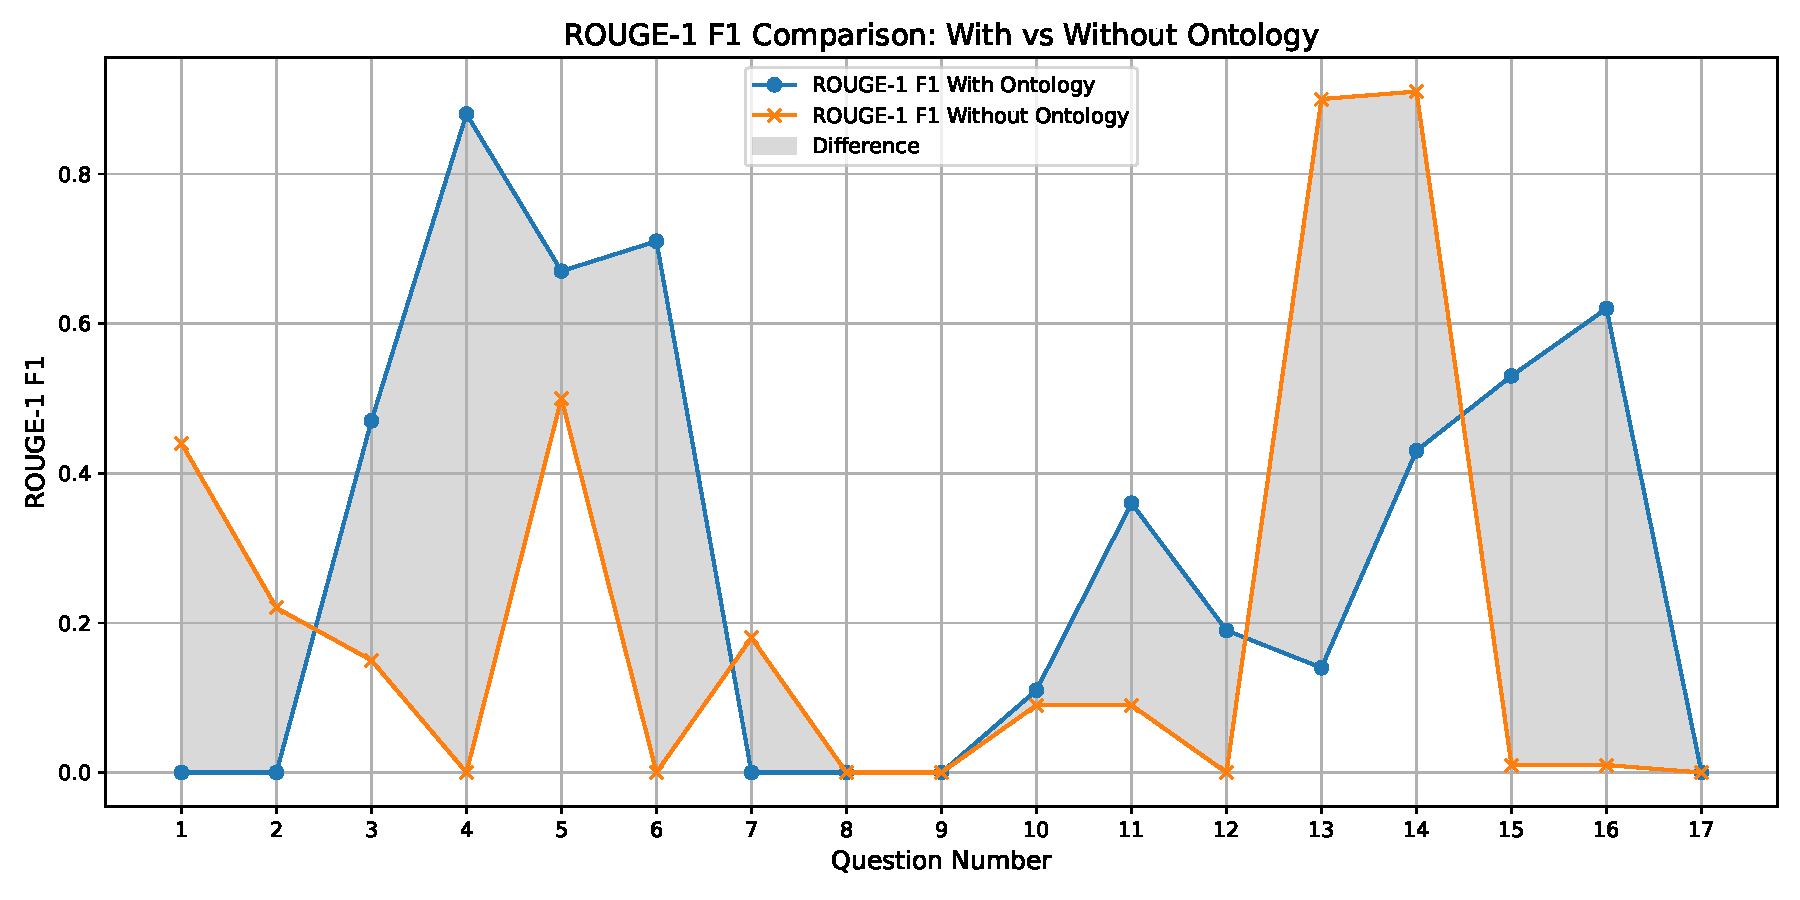
\includegraphics[width=0.8\textwidth]{{results/ROUGE-1_F1_Comparison.pdf}}
\caption{ROUGE-1 F1 Across Examples}
\end{figure}

\begin{figure}[h!]
\centering
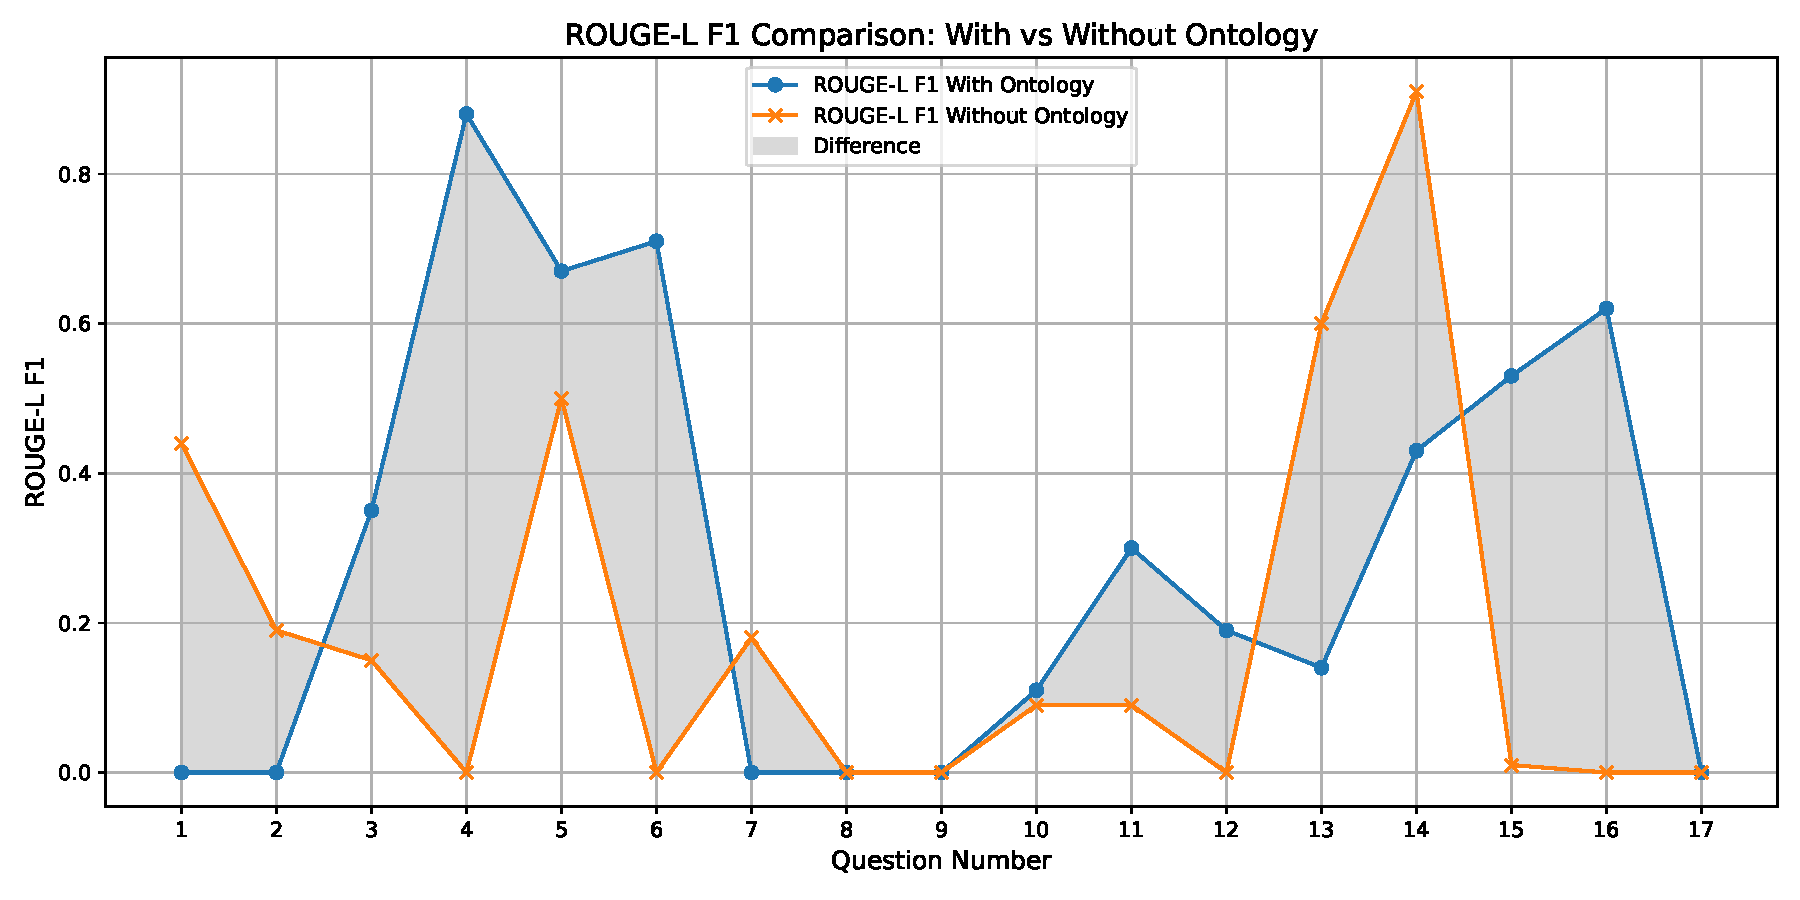
\includegraphics[width=0.8\textwidth]{{results/ROUGE-L_F1_Comparison.pdf}}
\caption{ROUGE-L F1 Across Examples}
\end{figure}

\begin{figure}[h!]
\centering
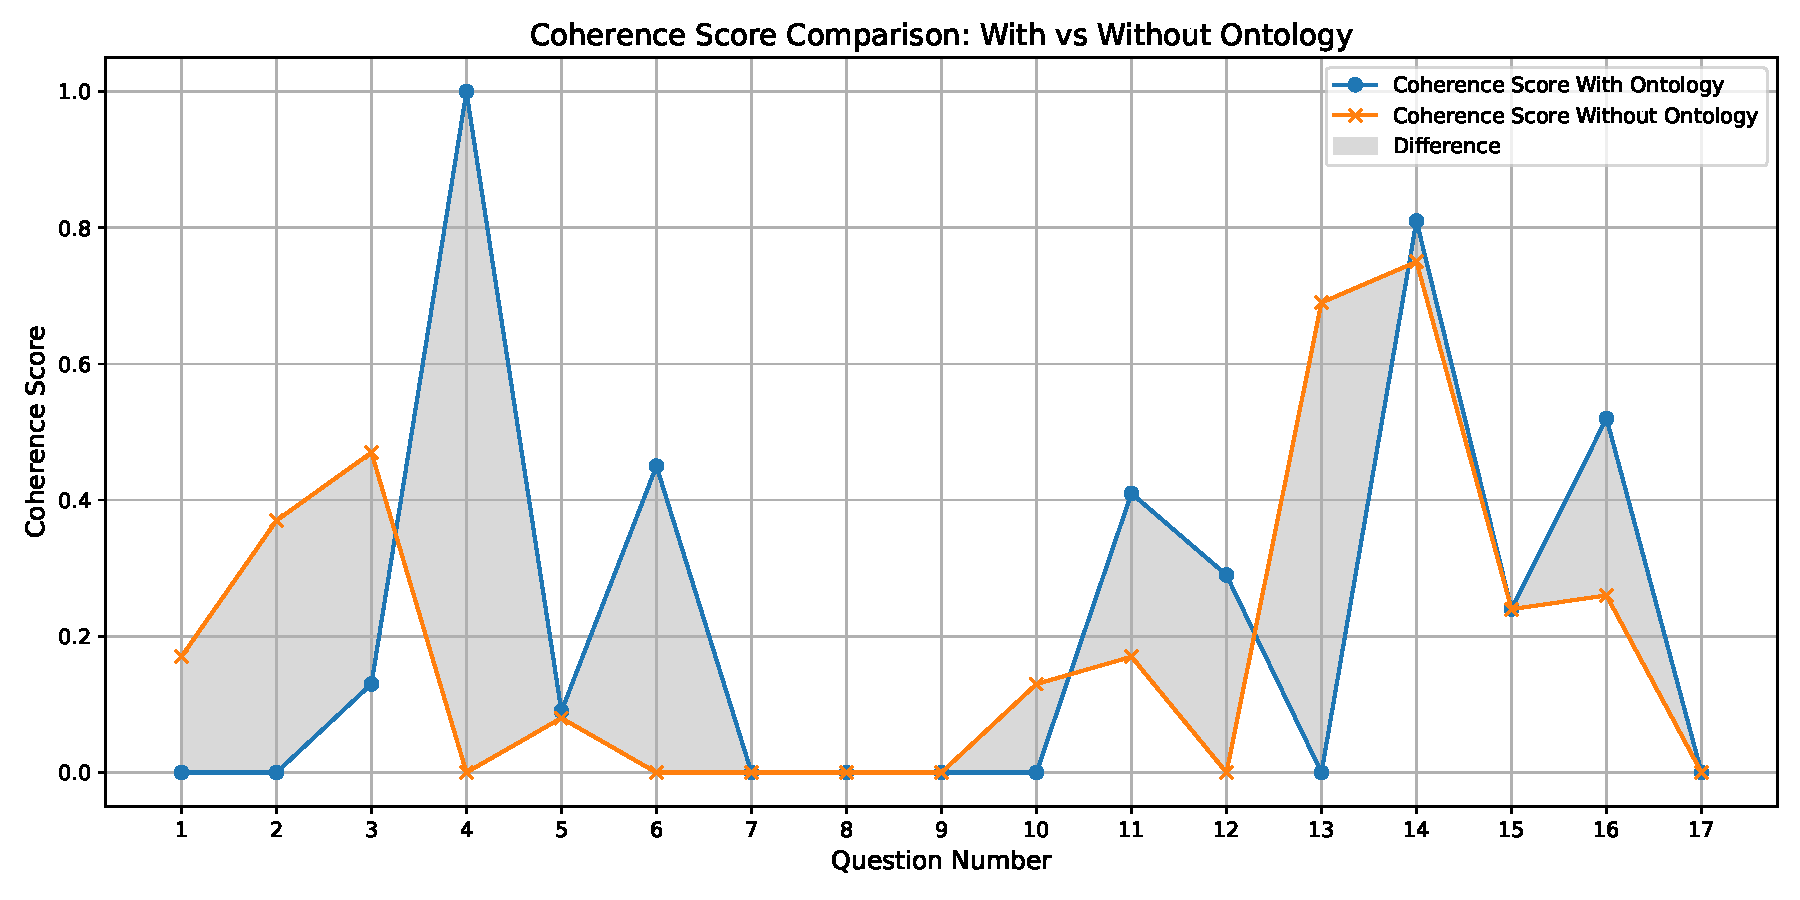
\includegraphics[width=0.8\textwidth]{{results/Coherence_Score_Comparison.pdf}}
\caption{Coherence Score Across Examples}
\end{figure}

\begin{figure}[h!]
\centering
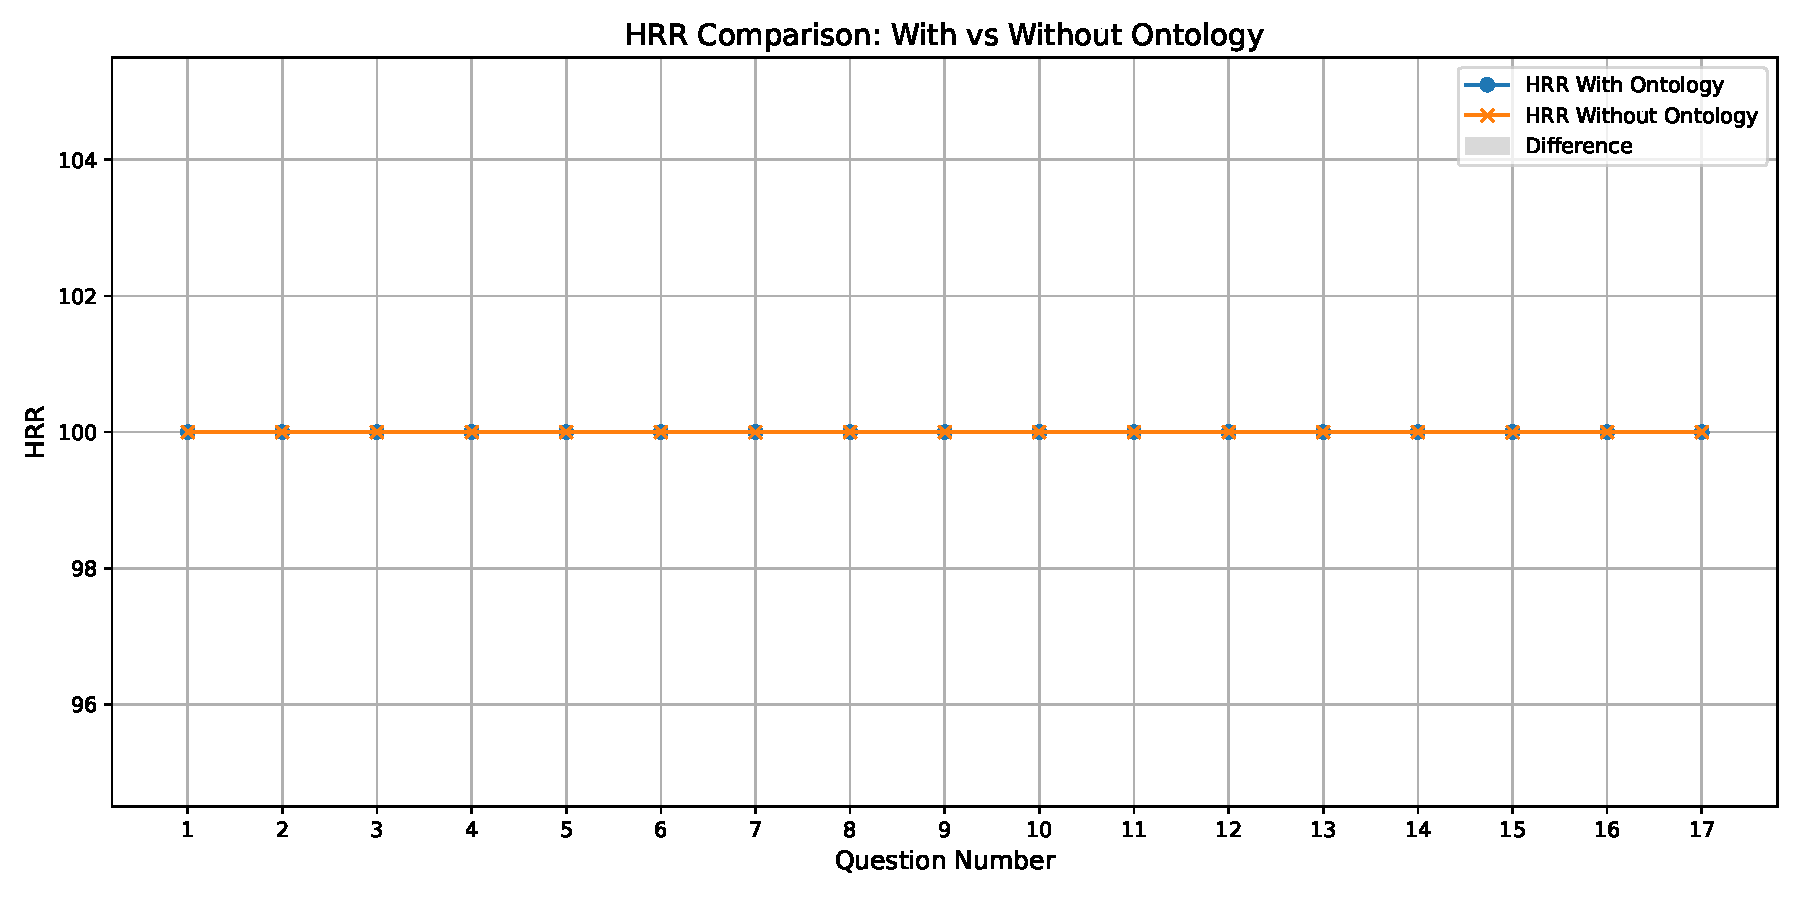
\includegraphics[width=0.8\textwidth]{{results/HRR_Comparison.pdf}}
\caption{HRR Across Examples}
\end{figure}

\begin{figure}[h!]
\centering
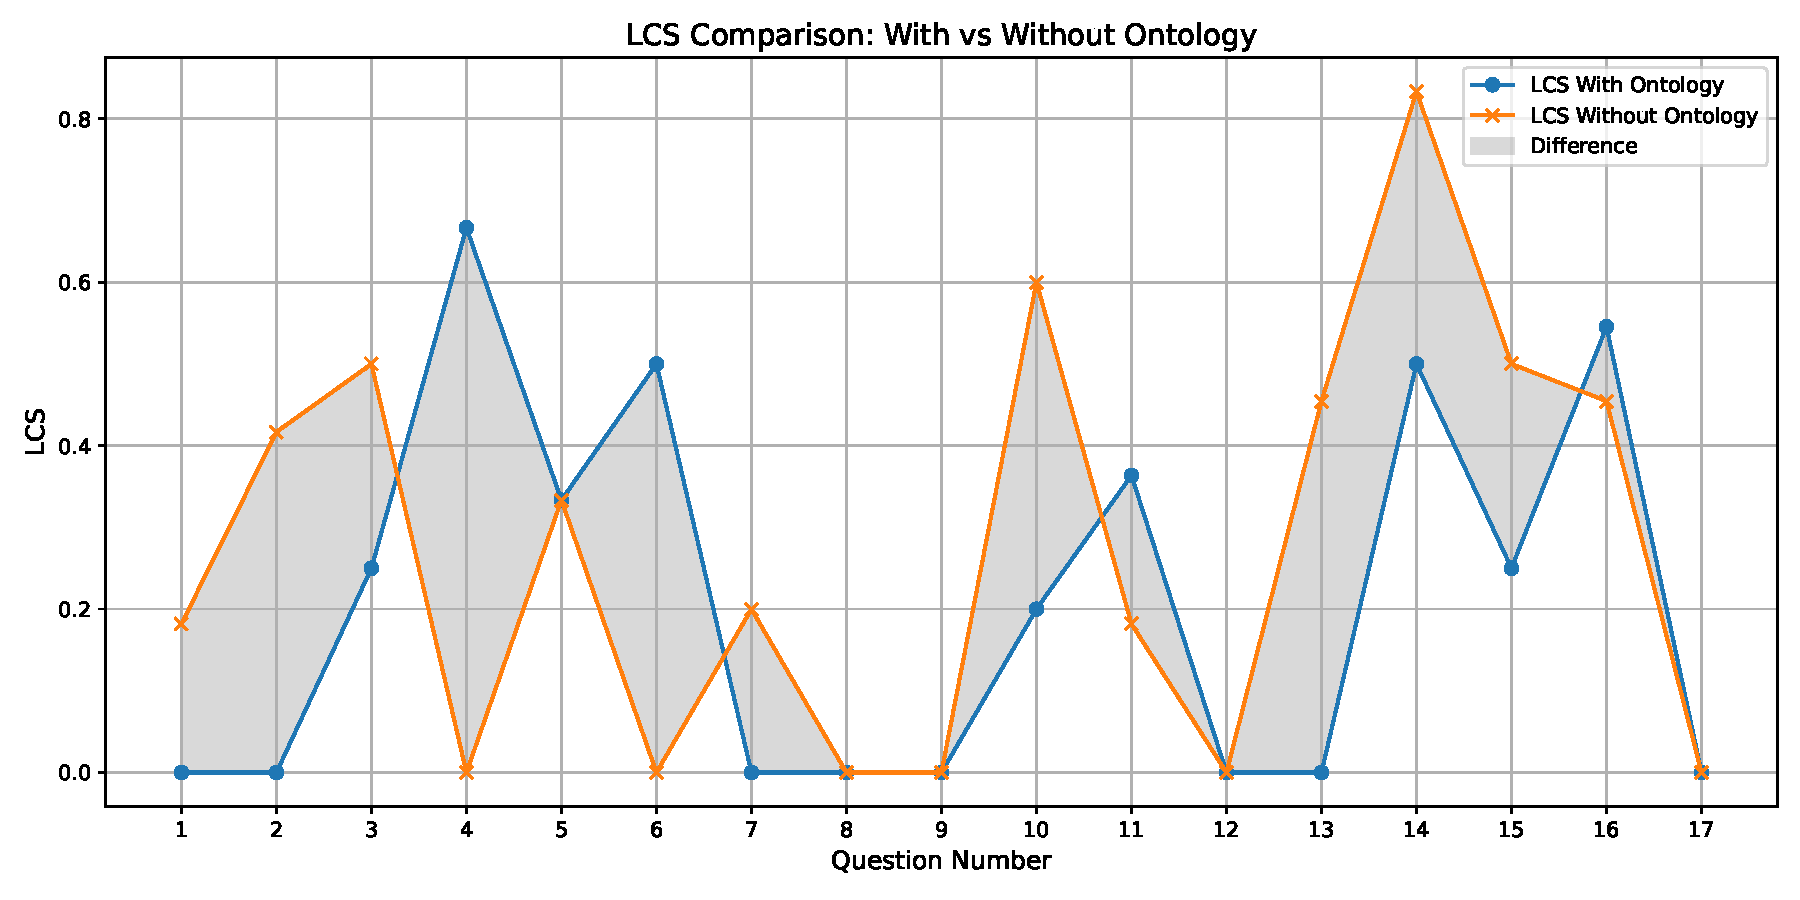
\includegraphics[width=0.8\textwidth]{{results/LCS_Comparison.pdf}}
\caption{LCS Across Examples}
\end{figure}

\begin{figure}[h!]
\centering
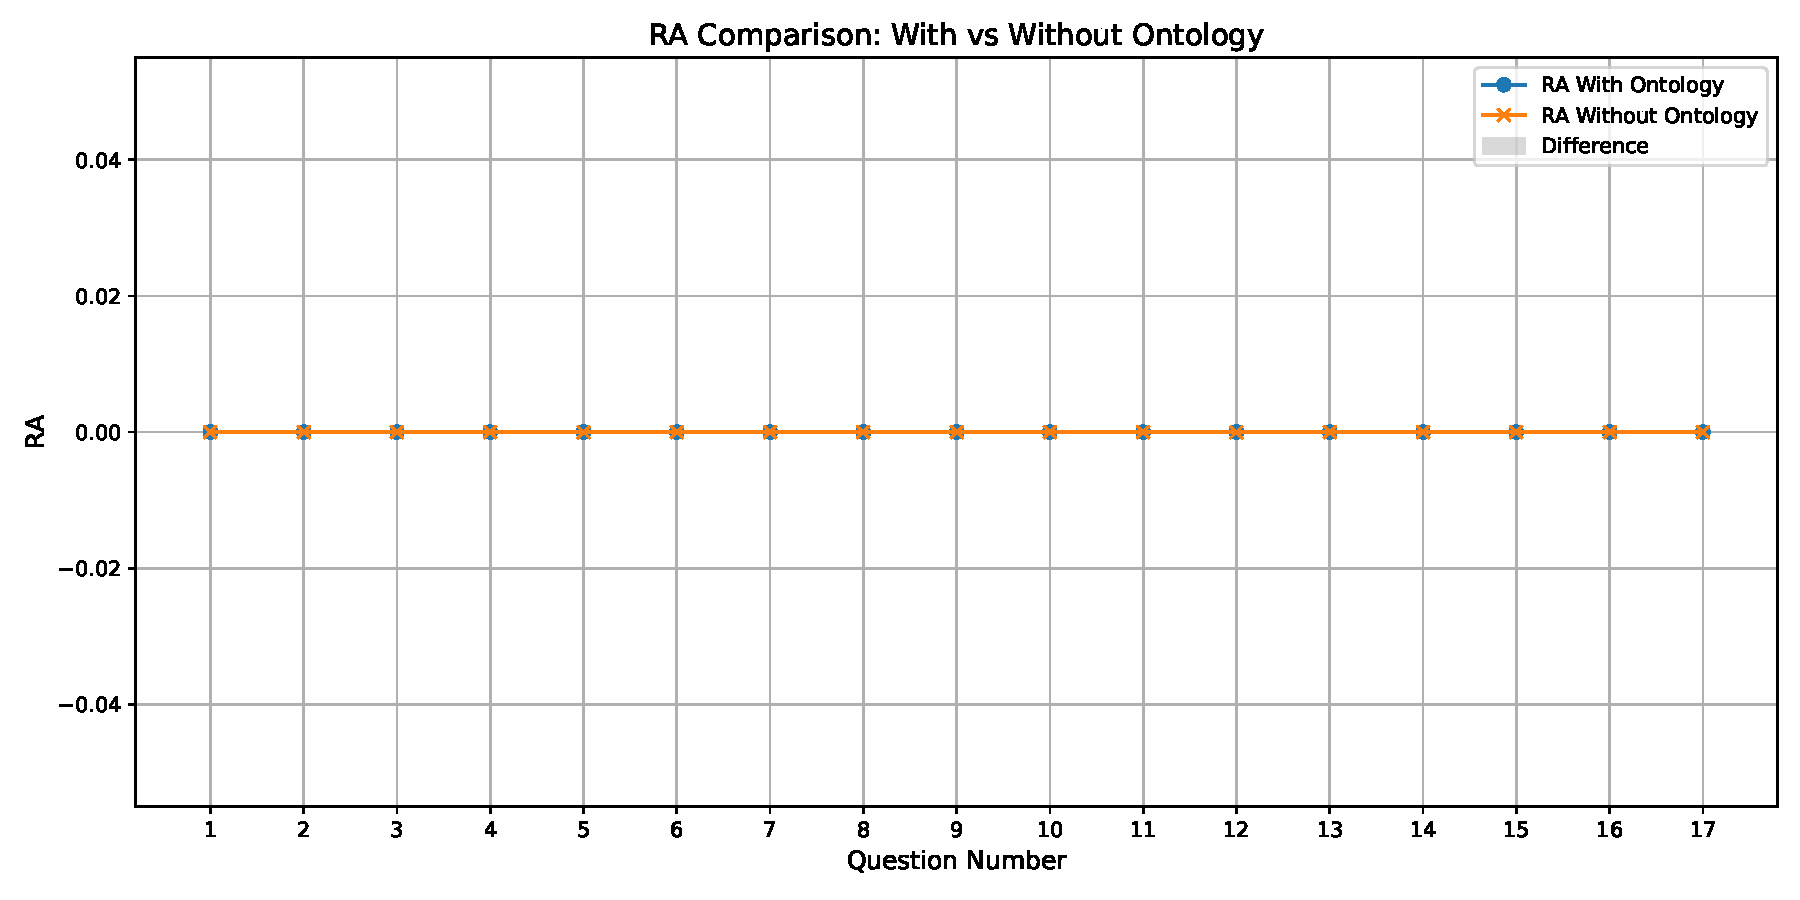
\includegraphics[width=0.8\textwidth]{{results/RA_Comparison.pdf}}
\caption{RA Across Examples}
\end{figure}

\begin{figure}[h!]
\centering
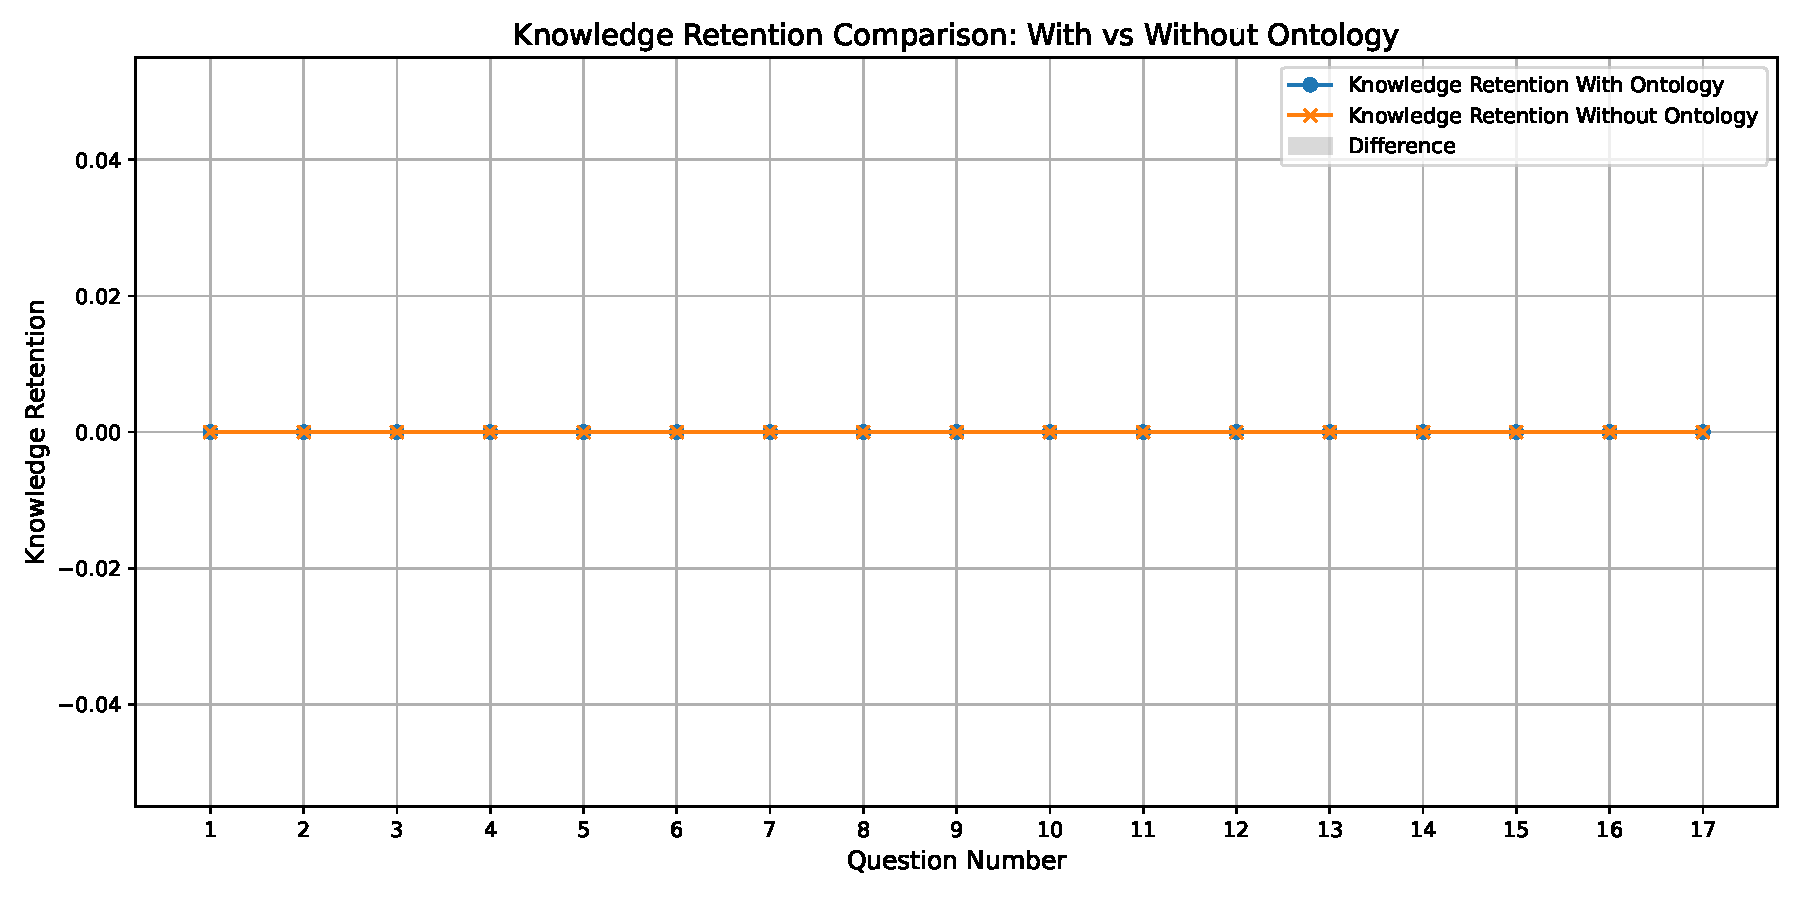
\includegraphics[width=0.8\textwidth]{{results/Knowledge_Retention_Comparison.pdf}}
\caption{Knowledge Retention Across Examples}
\end{figure}

\end{document}
